% Chapter 1

\chapter{Introduction}\label{Chapter1} % Main chapter title

 % For referencing the chapter elsewhere, use \ref{Chapter1} 

%----------------------------------------------------------------------------------------

% Define some commands to keep the formatting separated from the content 
\newcommand{\keyword}[1]{\textbf{#1}}
\newcommand{\tabhead}[1]{\textbf{#1}}
\newcommand{\code}[1]{\texttt{#1}}
\newcommand{\file}[1]{\texttt{\bfseries#1}}
\newcommand{\option}[1]{\texttt{\itshape#1}}

%\lhead{Chapter 1. \emph{Introduction}} 
%----------------------------------------------------------------------------------------
\textbf{Overview}\\
% \HRule \\[0.5cm]
\par\noindent\rule{\textwidth}{0.4pt}\\
\textit{This chapter introduces us to the general background of the research by briefly discussing the origin of the 21 cm radio line
and then moves on to discuss the significance of intensity mapping experiments. The research problems, key objectives, justification and the entire structure of the thesis 
are also outlined.}
\par\noindent\rule{\textwidth}{0.4pt}\\
% \HRule \\[1.5cm]
%
%  \enquote{spin-flip}
%----------------------------------------------------------------------------------------
\section{The 21 cm Radio Emission Line}	   \label{chap1:21cm}		
%%
% \vspace*{-2em}
Despite the fact that space is very empty and there is a great distance between the stars in the Milky Way, the gap between these
stars consists of dust and a very diffuse medium of gas. Astronomers refer to this matter and the radiation in space  as the \emph{interstellar medium} (ISM\footnote{\url{http://www-ssg.sr.unh.edu/ism/what1.html}}). The  interstellar gas can be found in molecular (mainly $\mathrm{H_{2}}$), ionic ($\mathrm{HII}$) or atomic (HI) form and 
it is composed of Hydrogen ($\approx 70\,\%$) followed by Helium ($\approx 28\,\%$) and the rest being heavy elements (Oxygen, Carbon and Nitrogen). 
The molecular and atomic Hydrogen gases are located in the colder dense regions of the ISM at ($T \sim {10-30}$)K and ($T \sim 50-100$)K respectively whilst, the ionic gas is in the warmer ($T \sim  {10^{3} - 10^{4}}$)K more dilute regions \citep{knee2001massive}.

% The simplest atom to understand among all the other kinds is the neutral hydrogen. It consists of a single proton and an electron with positive and negative charges respectively.
% These charges are attracted to each other by pulling the protons and the electrons together. 
% If the electron loses energy, then it moves closer to the proton, but if the electron gains energy, it is the vice versa. 
% Therefore, the energy released when an electron drops from a higher level to a lower level as shown in Fig.~\ref{fig:Hspin} (right  plot) 
% is known as the electromagnetic (EM) radiation. Depending on how far the electron has fallen, this can be a radio wave, visible light or even an
% ultra-violet. 
% %%

% Considering the neutral hydrogen (HI) atom in the Universe,
Nevertheless, a large portion of the hydrogen gas (mostly in atomic form) in the ISM is in the least energy state \citep{klessen2016physical}. 
Usually, both the proton and electron of a Hydrogen atom spin in the same state but, it happens very occasionally that (in every $11$ million years), 
the proton and the electron within the hydrogen atom 
will realign themselves slightly (that is, change the direction of the spin spontaneously) as shown in Fig.~\ref{fig:Hspin}, 
making the electrons to flip a little bit closer to the proton in a very specific way.
The fact that this is specific means that the frequency at which the EM radiation is given out is always the same, 
that is, the frequency is approximately $1420.406 \, \rm{MHz}$, and therefore, using large radio telescopes, radio
astronomers can observe the $21$ cm line (at  $1420.406$ MHz) even in very distant galaxies.
This 21 cm radio emission line was first proposed in the early 1940s by van de Hulst and is very famous in radio astronomy because 
it is the most powerful way of observing HI and making maps from it. 
Most often, when we observe the emission line, the distribution of this line  is Doppler shifted. This is because, a spiral galaxy rotates
in such a way that, if it is marginally edge-on to our line of sight, a portion of the HI regions
move away from us whilst others move towards us. This Doppler effect broadens the 21 cm
line into a double peak. It redshifts the radiation from the regions that move away from us
and blueshifts the vice versa.Therefore, the faster the rotation of the galaxy, the greater the
line broadening. It redshifts the radiation from the regions that move away from us
and blueshifts the vice versa.Therefore, the faster the rotation of the galaxy, the greater the
line broadening. Many academic works \citep{condon2016essential,wilson2013tools,wilson2009tools} give an in-depth explanation of this section.
% The unique wavelength this radiation has means we can actually detect the motion of the hydrogen compound to our motion. 
% This phenomenon is due to the Doppler effect. When a radio source is moving and giving out a signal or some
% kind of radiation, the fact that it is moving affects the frequency or the wavelength of that radiation. For instance, 
% relating this to our daily activities, when a siren or a car engine goes pass you, you will hear a change in the peak or tone. 
% Let assume a hydrogen atom is moving towards us and giving out radiation, then this radiation will be blueshifted with a shorter wavelength. 
% On the other hand, if the atom is moving away from us, it will be redshifted with a longer wavelength. This is really a useful extra piece of 
% information these observations give us. Using the redshift information, we will be able to determine distant galaxies in the universe. 

%%
\begin{figure}[ht]
	  \centering	     
	  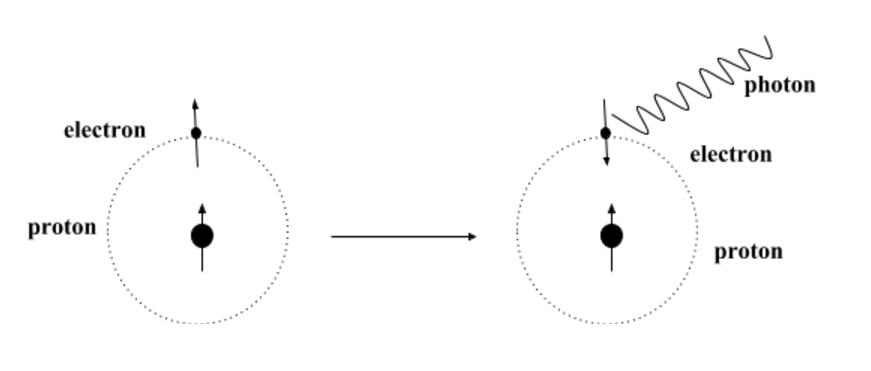
\includegraphics[width=3.8in]{c1/Hspin}	   
	  \caption{When the electron of a neutral hydrogen atom flips its spin, energy is released at a wavelength of $21\, \rm{cm}$. This figure is obtained from \cite[pg. 113]{ferrara2008first}.}
	  \label{fig:Hspin}
      \end{figure}
      \FloatBarrier
%%
The next section discusses how intensity mapping (IM) experiment is used to measure the distribution of the sky.

% %%
%----------------------------------------------------------------------------------------
% %

\section{HI Intensity Mapping} \label{chap1:h1mapping}
%%
The motivation to study cosmology in this present-day is to understand the massive size of the Universe, understand how the Universe expands and the distribution of everything. 
In order to do this, an observational time  is needed to really map out the large volume of data. Over the past two decades, the galaxy redshift surveys 
such as 2dF\footnote{\url{http://www.2dfgrs.net/}}, 6dF\footnote{\url{http://www-wfau.roe.ac.uk/6dFGS/}}, WiggleZ\footnote{\url{http://wigglez.swin.edu.au/site/}}, 
BOSS\footnote{\url{http://www.sdss3.org/surveys/boss.php}}, and SDSS\footnote{\url{http://www.sdss.org/}} 
use the optical spectroscopy to specifically observe millions of individual galaxies, determine each redshift and use these to estimate the energy distribution for each \citep{2009astro2010S.234P,1996ApJ...461...38S,1995ApJ...446..457S}. This approach really consumes a lot of time due to the map out of individual galaxies and also, it is very difficult to resolve faint sources. 
The total optical surveys used to localize the Universe in this way is approximately $1\%$ \citep{2009astro2010S.234P}.\\ %peterson200921}
%%
\indent Meanwhile, recent researches \citep{camera2014cosmology,2008PhRvL.100i1303C,2015aska.confE..19S,2015aska.confE..35W,2014MNRAS.441.3271W} on IM have shown that, this alternative approach does not resolve all the structures in the Universe but can actually provide us with a very good idea of how things are distributed as displayed in
Fig.~\ref{fig:implotb}. Here, the figure shows the variations in the simulated HI brightness temperature, where 
red indicates over-density and blue under-density, making it possible to infer from this map. From a cosmological point of view, that is sufficient enough because we can still see a lot of the features in Fig.~\ref{fig:implotb} map even though it's horribly pixelated as compared to Fig.~\ref{fig:implota}.
% %%
% 
\begin{figure}[H]
\begin{minipage}{\linewidth}
\centering
    \begin{subfigure}[b]{0.49\textwidth}
	      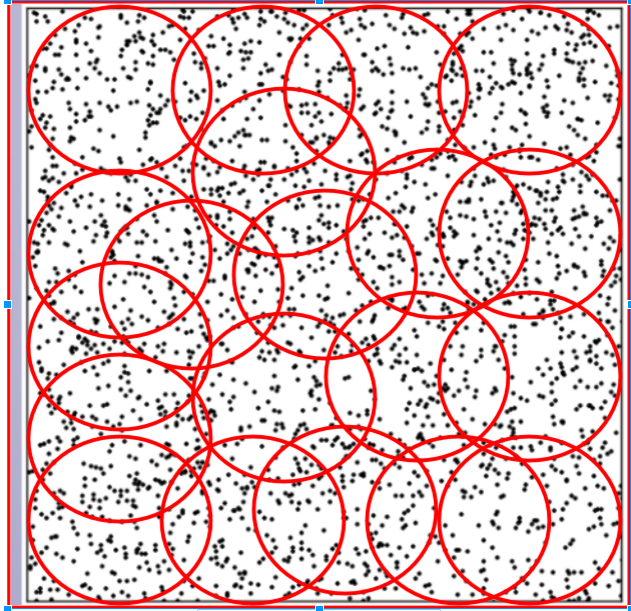
\includegraphics[width=\textwidth]{c1/g4}               
	      \caption{}                
	      \label{fig:implota}
      \end{subfigure}       
      \begin{subfigure}[b]{0.48\textwidth}
	      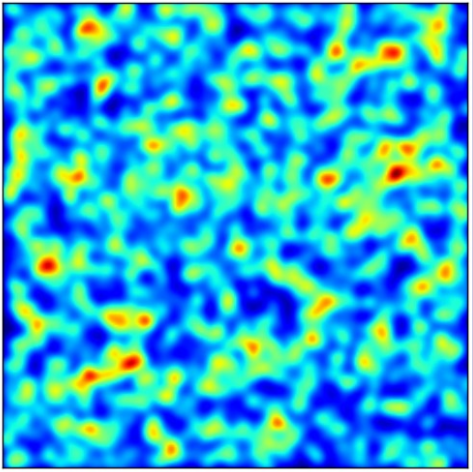
\includegraphics[width=\textwidth]{c1/g3}                
	      \caption{}               
	      \label{fig:implotb}
      \end{subfigure}        
	\end{minipage}
      \caption{Simulated variations in the 21 cm emission brightness temperature. The red rings in (a) show how to perform IM experiment by observing multiple patches in the sky with 
      the radio telescope in order to measure the 21 cm  emission to produce (b). Note that this figure is very similar to the one discussed in \citep{2009astro2010S.234P}.}%% \cite{peterson200921}
	\label{fig:implot}
\end{figure}
\FloatBarrier
% %

In terms of the observing strategy, a radio telescope (usually a big dish) is used to point and scan over the sky to measure the 21 cm spectral line. With this complementary approach, we can effectively map a large volume of the sky, since every frequency channel in the telescope will produce a different redshift of the HI. Note that, these big data obtained from the IM method can't really be achieved with any other method within the same period of time. These maps typically have a low spatial resolution, making it quite difficult to identify any single object as seen in Fig.~\ref{fig:implotb}. Nevertheless, the maps do have high redshift resolution due to the signal to noise in the instrument channels. Therefore, HI IM is the technique of integrating the spectral line flux over the whole HI mass function without selecting individual neutral objects.

Section~\ref{chap1:sec3} briefly discusses the importance of IM observational techniques and some of the current radio instruments purposely designed to perform this kind of experiment. 


% %%
% %----------------------------------------------------------------------------------------
% %%
% 
% %
\section{Significance of Intensity Mapping Techniques} \label{chap1:sec3}
%
The IM technique has the advantage of not resolving sources but instead measures diffuse sources that can be used to
generate tomographic maps of the Universe for many redshifts within the interval $0 < z < 6$ which is basically what the Square Kilometre Array (SKA) 
Phase I \citep{2010arXiv1008.2871G} is planning to do. In addition, the data produced from this technique contains spatial information that may be useful to 
measure Baryon Acoustic Oscillations (BAOs) \citep{2008PhRvL.100i1303C} which is one of the major incentive explored by the cosmologists and has led to the establishment of this method.
Measuring the BAOs for different redshifts would make us understand the expansion of the Universe. Furthermore, with the observational data from several lines, we
will also be able to cross-correlate the lines which can be used to remove the foreground from 21 cm observations. Finally,
the technique allows smaller and cheaper telescopes without long baselines such as HIRAX\footnote{{\url{https://www.acru.ukzn.ac.za/~hirax/}}}, to be used in such experiments,
hence increasing the science output in cosmology.\\
%%
\indent Presently, several IM experiments are in operation, such as the 
GBT\footnote{{\url{https://science.nrao.edu/facilities/gbt}}} (\enquote{Green Bank Telescope}), CHIME\footnote{{\url{https://chime-experiment.ca/}}} (\enquote{Canadian Hydrogen Intensity Mapping Experiment}),
Tianlai\footnote{{\url{http://tianlai.bao.ac.cn/}}} and FAST\footnote{{\url{http://fast.bao.ac.cn/en/}}} (\enquote{Five hundred metre Aperture Spherical Telescope}).
Among these instruments for IM experiments, the GBT produced the first HI signal at $z \sim 0.8$, using the cross-correlation of the redshift survey by WiggleZ 
\citep{chang2010intensity}. Moreover, the capabilities of upcoming instruments such as \enquote{dense aperture arrays for the  SKA} \citep{6051208} 
and HIRAX make it only more promising, due to the fact that, the technique is relatively \enquote{cheaper} compared to the usual galaxy surveys described 
in the first paragraph of Section~\ref{chap1:21cm}. Furthermore, these new instruments will provide a broader range of frequencies and a 
very massive survey area in order to produce HI intensity maps. Lastly, in IM, observations can be made at different redshifts either in single dish mode 
like BINGO \citep{battye2013h} or array mode like CHIME \citep{newburgh2014calibrating}.
%%
%  
% %----------------------------------------------------------------------------------------
% 
\section{Problem Identification} \label{chap1:sec4}
%
%
Radio telescopes are primarily used to intercept the signal coming from a radio source. During observation, the propagation effects and antenna feed electronics 
transform the measured signal. The direction-independent effects (DIEs) are described by the complex gains of each instrument as well as the receiver configuration. 
These effects are calibrated and corrected separately from imaging. However, the direction-dependent effects (DDEs) are much more complicated, 
since they are applied during imaging and therefore, are modified into a convolution of the measured components. This makes it 
very relevant to both calibrate the unknown DDE and then correct the known or measured one.
The ionospheric structure and the primary beam response of a two-axis mount telescope are the common sources of DDEs. They result in telescope mis-pointings
and antenna structure deformation caused by the gravitational loads acting on the dish and differential heating. These two time-varying terms go a long way to affect  
observations with the existing and upcoming instruments. For instance, the challenges put forward by ionospheric structure are particularly 
stern at very low frequencies and this can affect radio arrays like LOFAR\footnote{{\url{http://www.lofar.org/}}} \citep{2010ISPM...27...30W}. 
%%

Currently, the existing technique \citep{2015MNRAS.447..400A,2013ApJ...773...38G} used for IM requires a precise separation of the weak 21 cm line signal 
from the Galactic foreground continuum signal. This present approach is acceptable when there is  no instrumental distortion and the foreground signal is assumed
to be smooth.  However, DDEs are very crucial in physical observations and in IM experiments, the primary beam, in particular, is a challenge, 
as it modulates the intensity of the source with respect to the sky position, which is exactly what is being measured by this technique in the first place. 
In the case of Karoo Array Telescope (KAT-7\footnote{\url{http://public.ska.ac.za/kat-7}}), MeerKAT\footnote{\url{http://www.ska.ac.za/gallery/meerkat/}} and construction telescopes, these will be affected by pointing errors and DD polarization leakages. Present DD methods \citep{2011A&A...527A.106S} can not be used directly since distinct galaxies are not localized by this experiment. Hence, an improved method to resolve DDEs in a stochastic way has to be developed.
%%
%

\section{Research Objective} \label{chap1:sec5}
%%%
The key focus of this project is to develop IM techniques for mapping out primary beams of a radio telescope and then, introducing realistic errors to perturb these modelled beams.
We then attempt a correction and calibration of these distorted modelled beams and ultimately, use the final data for intensity mapping experiments. Thus, we use
these modelled beams to simulate  the complete-sky maps and then, determine the foregrounds that have corrupted the total intensity due to polarization leakage and errors in the primary beams which
have not been accounted for. The study used Oxford's Square Kilometre Array Radio-telescope (\texttt{OSKAR}\footnote{\url{http://www.oerc.ox.ac.uk/~ska/oskar2/}}),
a beamforming simulator, specifically developed to generate simulated data from large aperture arrays, such as those envisaged for the SKA Phase I, to simulate the KAT-7
notional beams. The next beams produced for this study are Zernike models reconstructed from MeerKAT holography measured beams. 
The last primary beams used in this research are obtained from the Generalized Reflector Antenna farm analysis Software Package
(\texttt{GRASP}\footnote{\url{ http://www.ticra.com/products/software/grasp}}) of electromagneTIC RAdiation (\texttt{TICRA}) software.

In addition, apart from studying the $21\, \rm{cm}$ line, there are other spectral lines such as 
CII fine-structure line \citep{2012ApJ...745...49G,2015ApJ...806..209S,2015MNRAS.450.3829Y},
Ly$\alpha$ line \citep{2017MNRAS.464..469S,Tapken:2007ja,2015ApJ...810L..12Z}, and the rotational CO lines \citep{Lidz:2011dx,padmanabhan2017constraining,vallini2017co} that detect
different physical mechanisms. Therefore, this work will use the SKA1-mid to look into CO IM for high redshift in conjunction with HI IM at low redshift. Details of this
will be discussed in Chapter~\ref{Chapter6}.
%----------------------------------------------------------------------------------------

\section{Delimitation} \label{chap1:sec6}
%
The study's main scope is to calibrate two outcomes: 
\begin{enumerate}[label=(\roman*)]
\item the effect of polarization leakage to the estimated HI and CO spectra, using realistic primary beams and \label{itm:first}
\item the inaccuracies in the estimate of~\ref{itm:first} due to the perturbations that have not been modelled in the primary beams.
\end{enumerate}
% 
% 
% %----------------------------------------------------------------------------------------

\section{Rationale and Motivation} 	\label{chap1:sec7}
%%%
Normally, when a portion of two signals leak into each other due to inadequacies in the mechanical and electrical designs of the antenna, it is referred to as the
\emph{polarization leakage}. With regard to Stokes parameters, this creates an undesired spread of the signal from the absolute intensity $I$ to polarization $QUV$  and vice-versa.
This problem is  very unique in IM experiments and since Faraday effect rotates the polarization $QU$, the polarized foregrounds are generally not uniform across 
frequency \citep{doi:10.1093/mnras/stv1107}. This challenge can go a long way to limit observations not only with the present working telescopes but even those under construction.   
The study is motivated by this and therefore, concentrates rather on the effects of the primary beam particularly, DD polarization leakage. The potential of IM has already been demonstrated \citep{2015aska.confE..35W,2008PhRvL.100i1303C,2014MNRAS.441.3271W,2008PhRvL.100p1301L,2015aska.confE..19S} and the capabilities of upcoming telescopes as mentioned in Section~\ref{chap1:sec3} make it only more promising. However, considerable research into this
technique is necessary since there are some sort of technical challenges in terms of data analysis and in particular measuring the primary beam response, which has to be overcome in order to make such an experiment work to its full potential.
%
% %---------------------------------------------------------------------------------------------------------------------------------------

\section{Thesis Layout}	 \label{chap1:sec8}
%
The study is divided into seven different chapters as follows:

Chapter~\ref{Chapter1} briefly introduces the research topic by commencing with the general background of 21 cm emission line and continues by
presenting the significance of IM experiment and clearly stating the research problem and objective. This chapter also justifies why the study is conducted 
and briefly explains how the simulations are done to produce the primary beams for various antenna types.

%   %%
Chapter~\ref{Chapter2} discusses radio telescope antennas, where we clearly look at the numerous designs, operations and performances of antennas. 
Radio array types and the concept of measurement equation are also reviewed in this chapter.  


Foregrounds and rotation measure synthesis are discussed in Chapter~\ref{Chapter3}. Here, the study mainly focused on synchrotron
emission and concisely describe how we simulate the foreground and applied rotational measures. 


Chapter~\ref{Chapter4} presents the first methodology employed in this research. In this chapter, we describe extensively the observational effects of primary beam perturbation 
of KAT-7, using the {\tt OSKAR} software package. We then go ahead to determine the polarization leakage by introducing the convolution technique to simulate the foregrounds produced 
in Chapter~\ref{Chapter3}. Here, KAT-7 is used as a conceptual example for the purposes of this study. The study moves on further to compare the energy profile of the  simulated beams and the  Jansky Very Large Array (JVLA\footnote{\url{https://science.nrao.edu/facilities/vla}}) holography measured beams. 
%%

Chapter~\ref{Chapter5} describes the second methodology of this study. In this chapter, we produce modelled beams by fitting Zernike polynomials on MeerKAT measured beams 
to compute the reconstructed beams with fewer coefficients. We then estimate the effect on IM by measuring the foregrounds in Chapter~\ref{Chapter3} with the Zernike-beams.

The third methodology in this work is presented in Chapter~\ref{Chapter6}, where we generate {\tt GRASP} simulated EM beams of SKA1-mid for bands $1, 2$ and $5$. 
These EM beams of various bands are reconstructed with the Zernike model, using the strongest Zernike coefficients (that is, selected number of coefficients) and in addition, 
we try to perturb these {\tt GRASP} beams by introducing errors in the feed coordinates to displace the feed from its principal focus. 
Finally, we perfom IM experiments by simulating the foregrounds in Chapter~\ref{Chapter3} with all these modelled beams to estimate not only HI flux at lower bands 
but also CO signals too at higher bands.
%%


Conclusions and recommendations are discussed in Chapter~\ref{Chapter7}.
%%
